\documentclass[a4paper]{book}
\usepackage{a4wide}
\usepackage{makeidx}
\usepackage{fancyhdr}
\usepackage{graphicx}
\usepackage{multicol}
\usepackage{float}
\usepackage{textcomp}
\usepackage{alltt}
\usepackage{doxygen}
\makeindex
\setcounter{tocdepth}{1}
\renewcommand{\footrulewidth}{0.4pt}
\begin{document}
\begin{titlepage}
\vspace*{3cm}
\begin{center}

{\Large \textbf{The GENIE Object Oriented Neutrino Generator}}\\
\vspace*{1cm}
{\Large \textbf{REFERENCE MANUAL}}\\
\vspace*{1cm}

{\large \textbf{Generated by Doxygen 1.4.0}}\\
\vspace*{0.5cm}
{\large \today}\\
\vspace*{1cm}

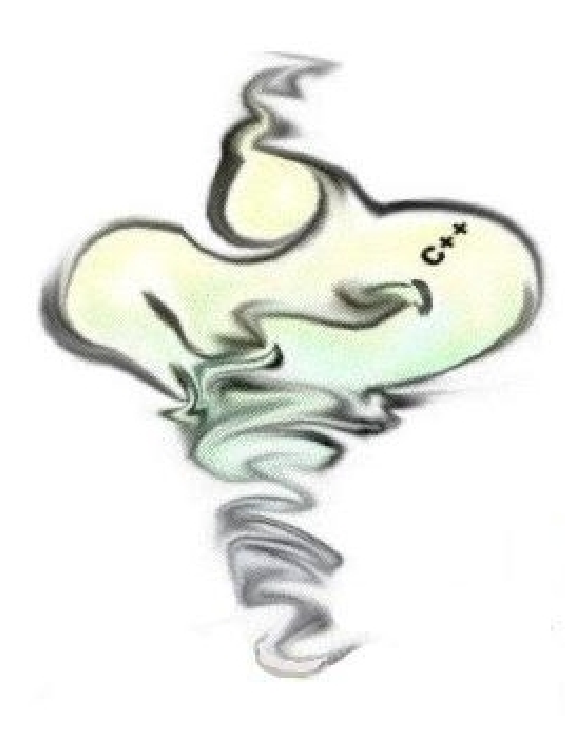
\includegraphics[width=5cm,keepaspectratio]{../../data/logo/genie_logo.eps}

\vspace*{0.6cm}

{\textbf{Costas Andreopoulos$^{2}$, Flavio Cavanna$^{7}$ Jerome Damet$^{6}$, Hugh Gallagher$^{9}$,
Yoshinari Hayato$^{5}$, Stefan Kretzer$^{1}$, Anselmo Meregaglia$^{4}$,
Donna Naples$^{8}$, Geoff Pearce$^{2}$, Andre Rubbia$^{4}$, Mike Whalley$^{3}$}}\\
\vspace*{0.5cm}

{\textit{$^{1}$Brookhaven National Laboratory, $^{2}$CCLRC - Rutherford Appleton Laboratory,
$^{3}$Durham University, $^{4}$ETH Zurich, $^{5}$Kamioka Observatory, ICRR, University of Tokyo, 
$^{6}$Laboratoire d'Annecy le vieux de Physique des Particules, $^{7}$L'Aquila University/ INFN, 
$^{8}$Pittsburgh University, $^{9}$Tufts University}}

\end{center}
\end{titlepage}
\clearemptydoublepage
\pagenumbering{roman}
\tableofcontents
\clearemptydoublepage
\pagenumbering{arabic}
